\newpage
\appendix
\newpage

\captionsetup[figure]{font=small,skip=0pt}
\etocdepthtag.toc{mtappendix}
\etocsettagdepth{mtchapter}{none}
\etocsettagdepth{mtappendix}{subsection}
\etoctocstyle{1}{Appendix - Contents}
\tableofcontents
\pagestyle{plain}
\newpage
\pagenumbering{arabic}

\chapter{Detailed Explanations and Supplementary Results}
In this chapter, the detailed explanations of the concepts discussed in the main text and present supplementary results that contribute to a clearer overview of the key outcomes of this thesis. These additional findings provide valuable context and insights that complement the primary research findings.

\section{Quaternions to Euler Angles}
\label{sec:Q2E}
Even though Euler angles are used to represent rotations, the transmission of two poses are calculated by Quaternion, which is a mathematical construct that extends the notion of complex numbers to four dimensions. They comprise four components: a scalar part represented by $w$, and a vector component denoted as $\vec{v}=(x, y, z)$. Quaternions are expressed as:
$$q = w + xi + yj + zk$$
where $x$, $y$, $z$, and $w$ are real numbers, and $i$, $j$, and $k$ are three imaginary units that satisfy the following multiplication rules: $i^2 = j^2 = k^2 = ijk = -1$. This approach involves establishing the initial pose of the robot as a quaternion and subsequently updating the current pose through sensors like accelerometers and gyroscopes. By computing the difference between the initial and current poses, the rotational component of the transformation can be extracted. This rotational component is often represented as a 3x3 rotation matrix $R$, which can then be used to derive the Euler angles 'yaw', 'pitch', and 'roll', providing insights into the robot's orientation in three-dimensional space. 
$$ R = \begin{bmatrix}
1 - 2(y^2 + z^2) & 2(xy - wz) & 2(xz + wy) \\
2(xy + wz) & 1 - 2(x^2 + z^2) & 2(yz - wx) \\
2(xz - wy) & 2(yz + wx) & 1 - 2(x^2 + y^2)
\end{bmatrix}
$$
The conversion from the rotation matrix 'R' to Euler angles 'yaw', 'pitch', and 'roll' involves the following mathematical expressions:
\begin{align*}
\text{yaw (Y)} & = \text{atan2}(R_{21}, R_{11}) \\
\text{pitch (X)} & = -\text{asin}(R_{31}) \\
\text{roll (Z)} & = \text{atan2}(R_{32}, R_{33})
\end{align*}

\section{Kalman Filter Update}
\label{sec:kf}
The Kalman filter, a fundamental tool in state estimation for dynamic systems, continuously refines its state estimate in the presence of noisy measurements. This section provides an overview of the Kalman filter's update process, shedding light on its predictive and corrective steps.

\textbf{State Transition Model (Predictive Step):}
In the predictive step, the Kalman filter employs the system's dynamics to forecast the next state ($x_{k|k-1}$) based on the previous state estimate ($x_{k-1|k-1}$). This forecast hinges on a linear transformation captured by the state transition matrix ($A$):
\begin{equation*}
x_{k|k-1} = A \cdot x_{k-1|k-1}
\end{equation*}

The state covariance ($P_{k|k-1}$) is also updated to account for the inherent uncertainty in this prediction:
\begin{equation*}
P_{k|k-1} = A \cdot P_{k-1|k-1} \cdot A^T + Q
\end{equation*}
Here, $Q$ represents the process noise covariance matrix, characterizing the uncertainty introduced by the system dynamics.

\textbf{Measurement Update (Corrective Step):}
In the corrective step, measurements ($z_k$) are incorporated into the state estimate to enhance its accuracy. The Kalman gain ($K_k$) is computed to determine the weight assigned to the measurement versus the prediction:
\begin{equation*}
K_k = P_{k|k-1} \cdot H^T \cdot (H \cdot P_{k|k-1} \cdot H^T + R)^{-1}
\end{equation*}
In this equation, $H$ represents the measurement matrix, mapping the state to the measurement space. The measurement noise covariance matrix ($R$) captures the uncertainty associated with sensor measurements.

Leveraging the Kalman gain, the state estimate and its covariance are updated as follows:
\begin{align*}
x_{k|k} = x_{k|k-1} + K_k \cdot (z_k - H \cdot x_{k|k-1}) \
P_{k|k} = (I - K_k \cdot H) \cdot P_{k|k-1}
\end{align*}
In these equations, $I$ denotes the identity matrix. The Kalman filter's iterative process continually refines the state estimate and its associated uncertainty, making it a powerful tool for state estimation in the presence of noise and uncertainty..

\section{Single Step Prediction of two NNs}
\begin{figure}[htb]
    \centering
    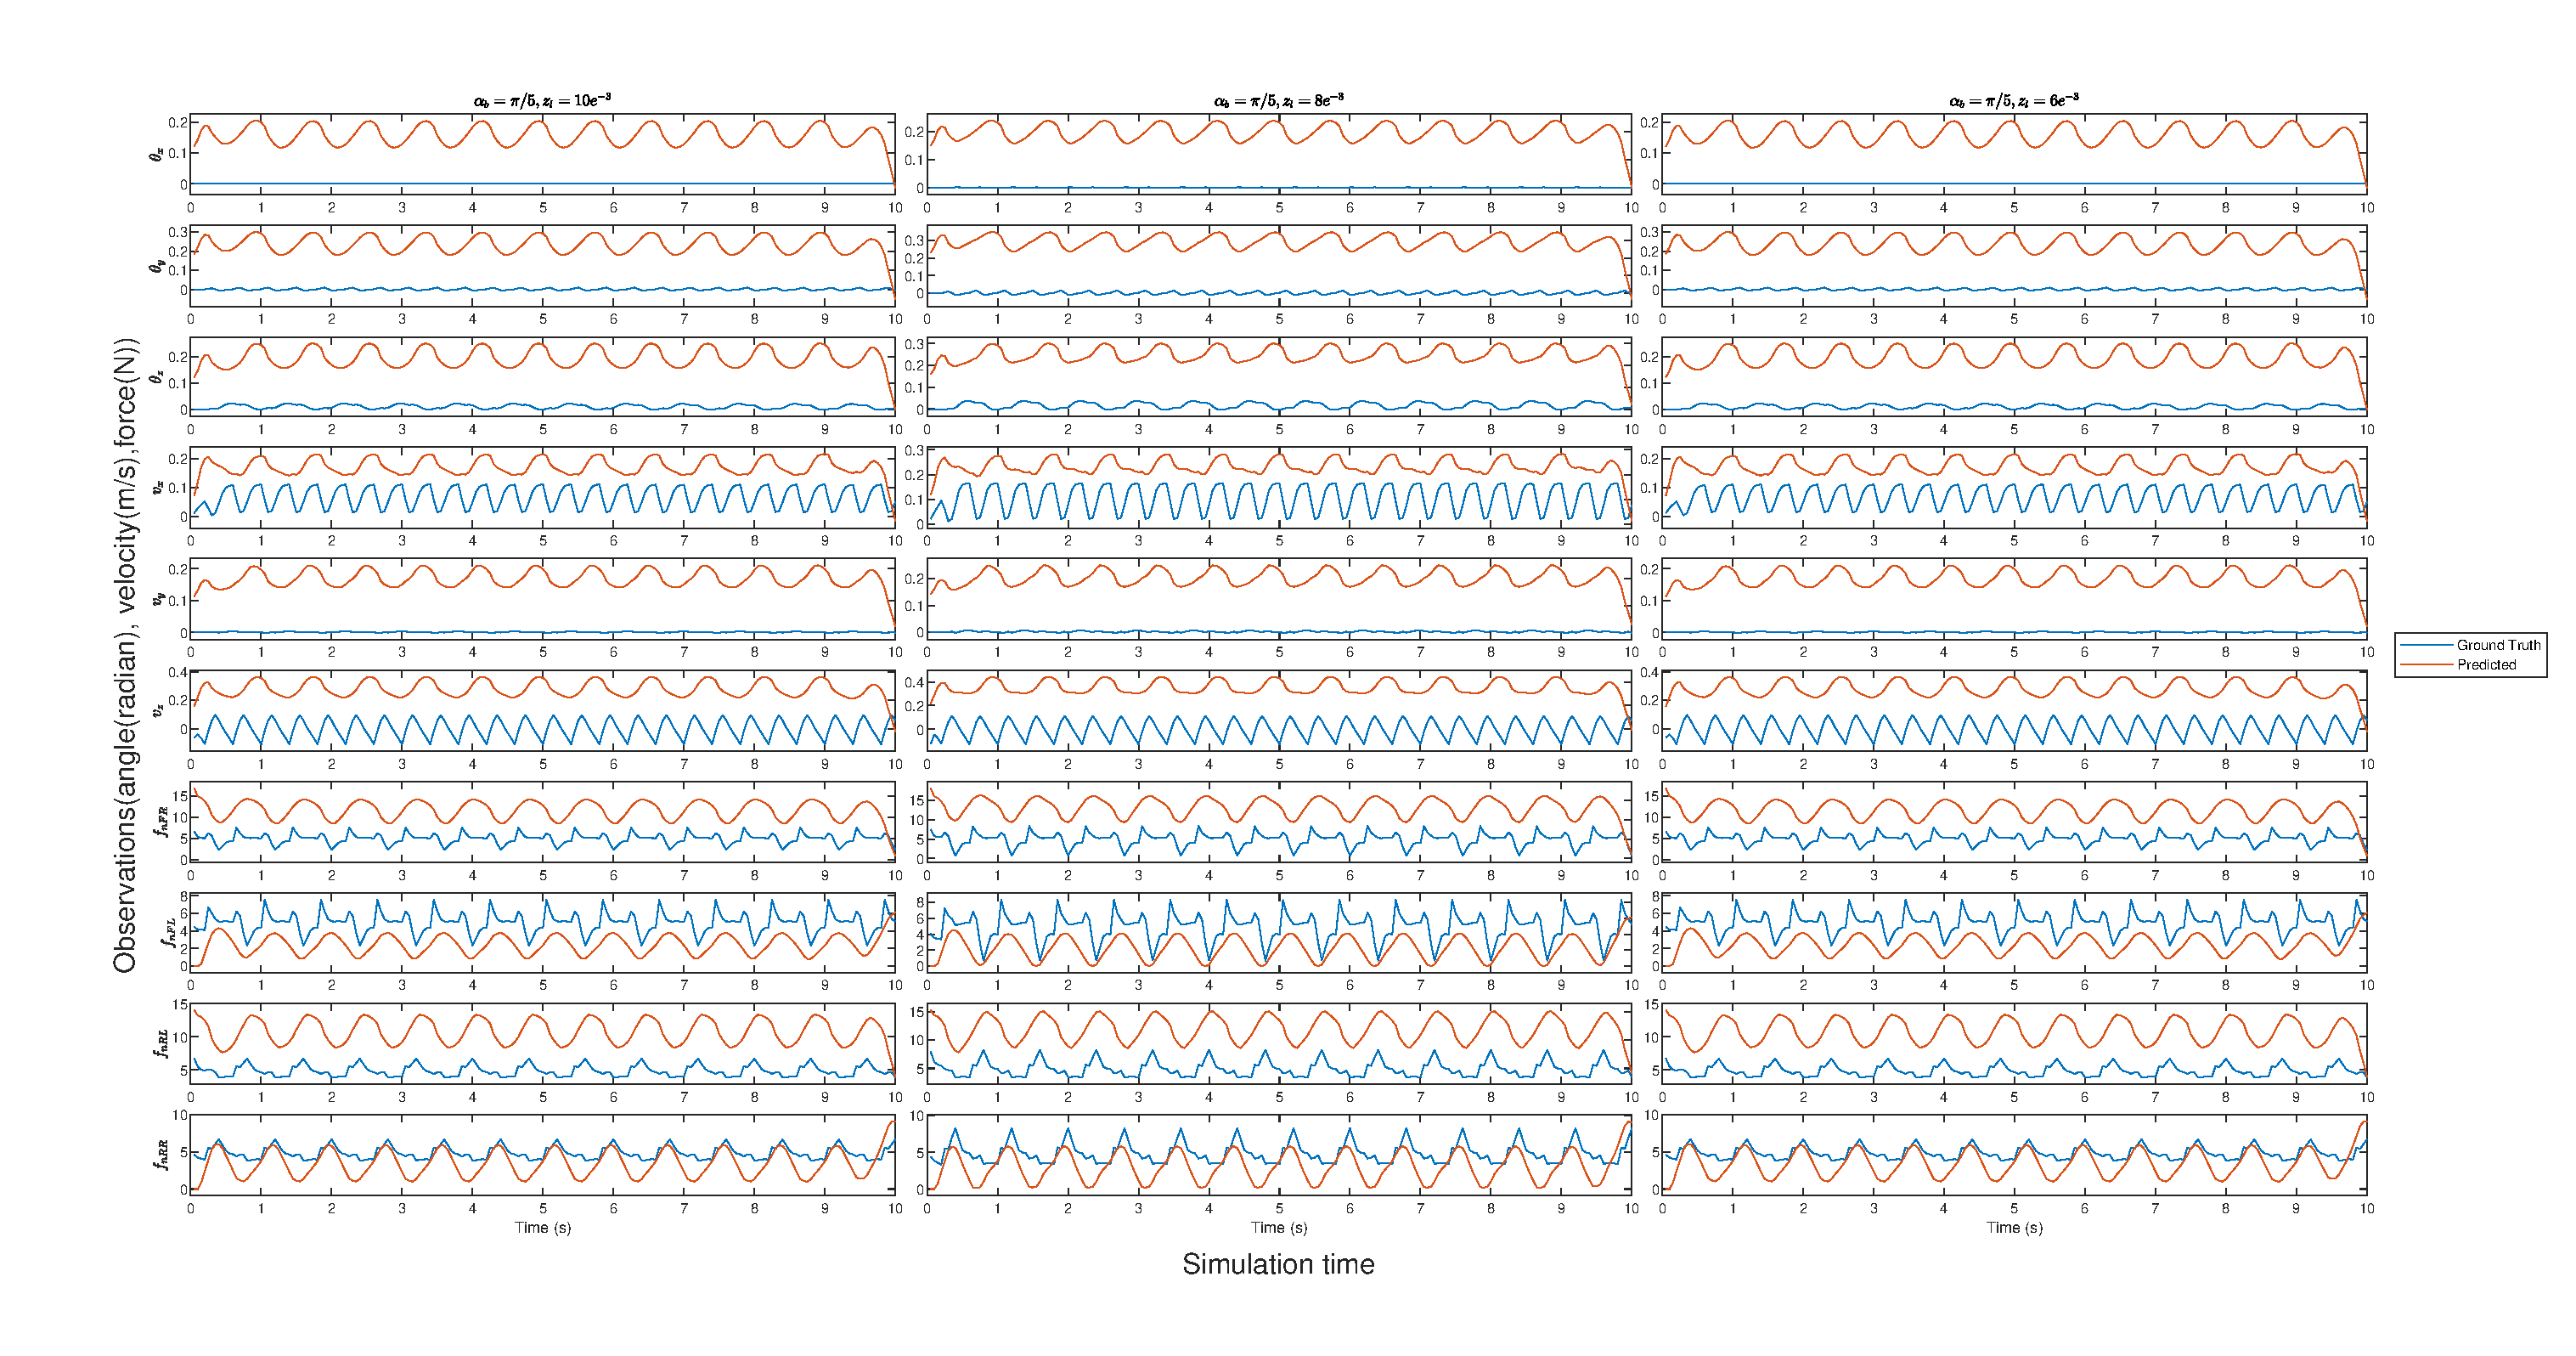
\includegraphics[width=\linewidth]{img/AppA/lstm_pred.eps}
    \caption{Single step prediction test of LSTM network}
    \label{fig:lstm_test}
\end{figure}

\begin{figure}[htb]
    \centering
    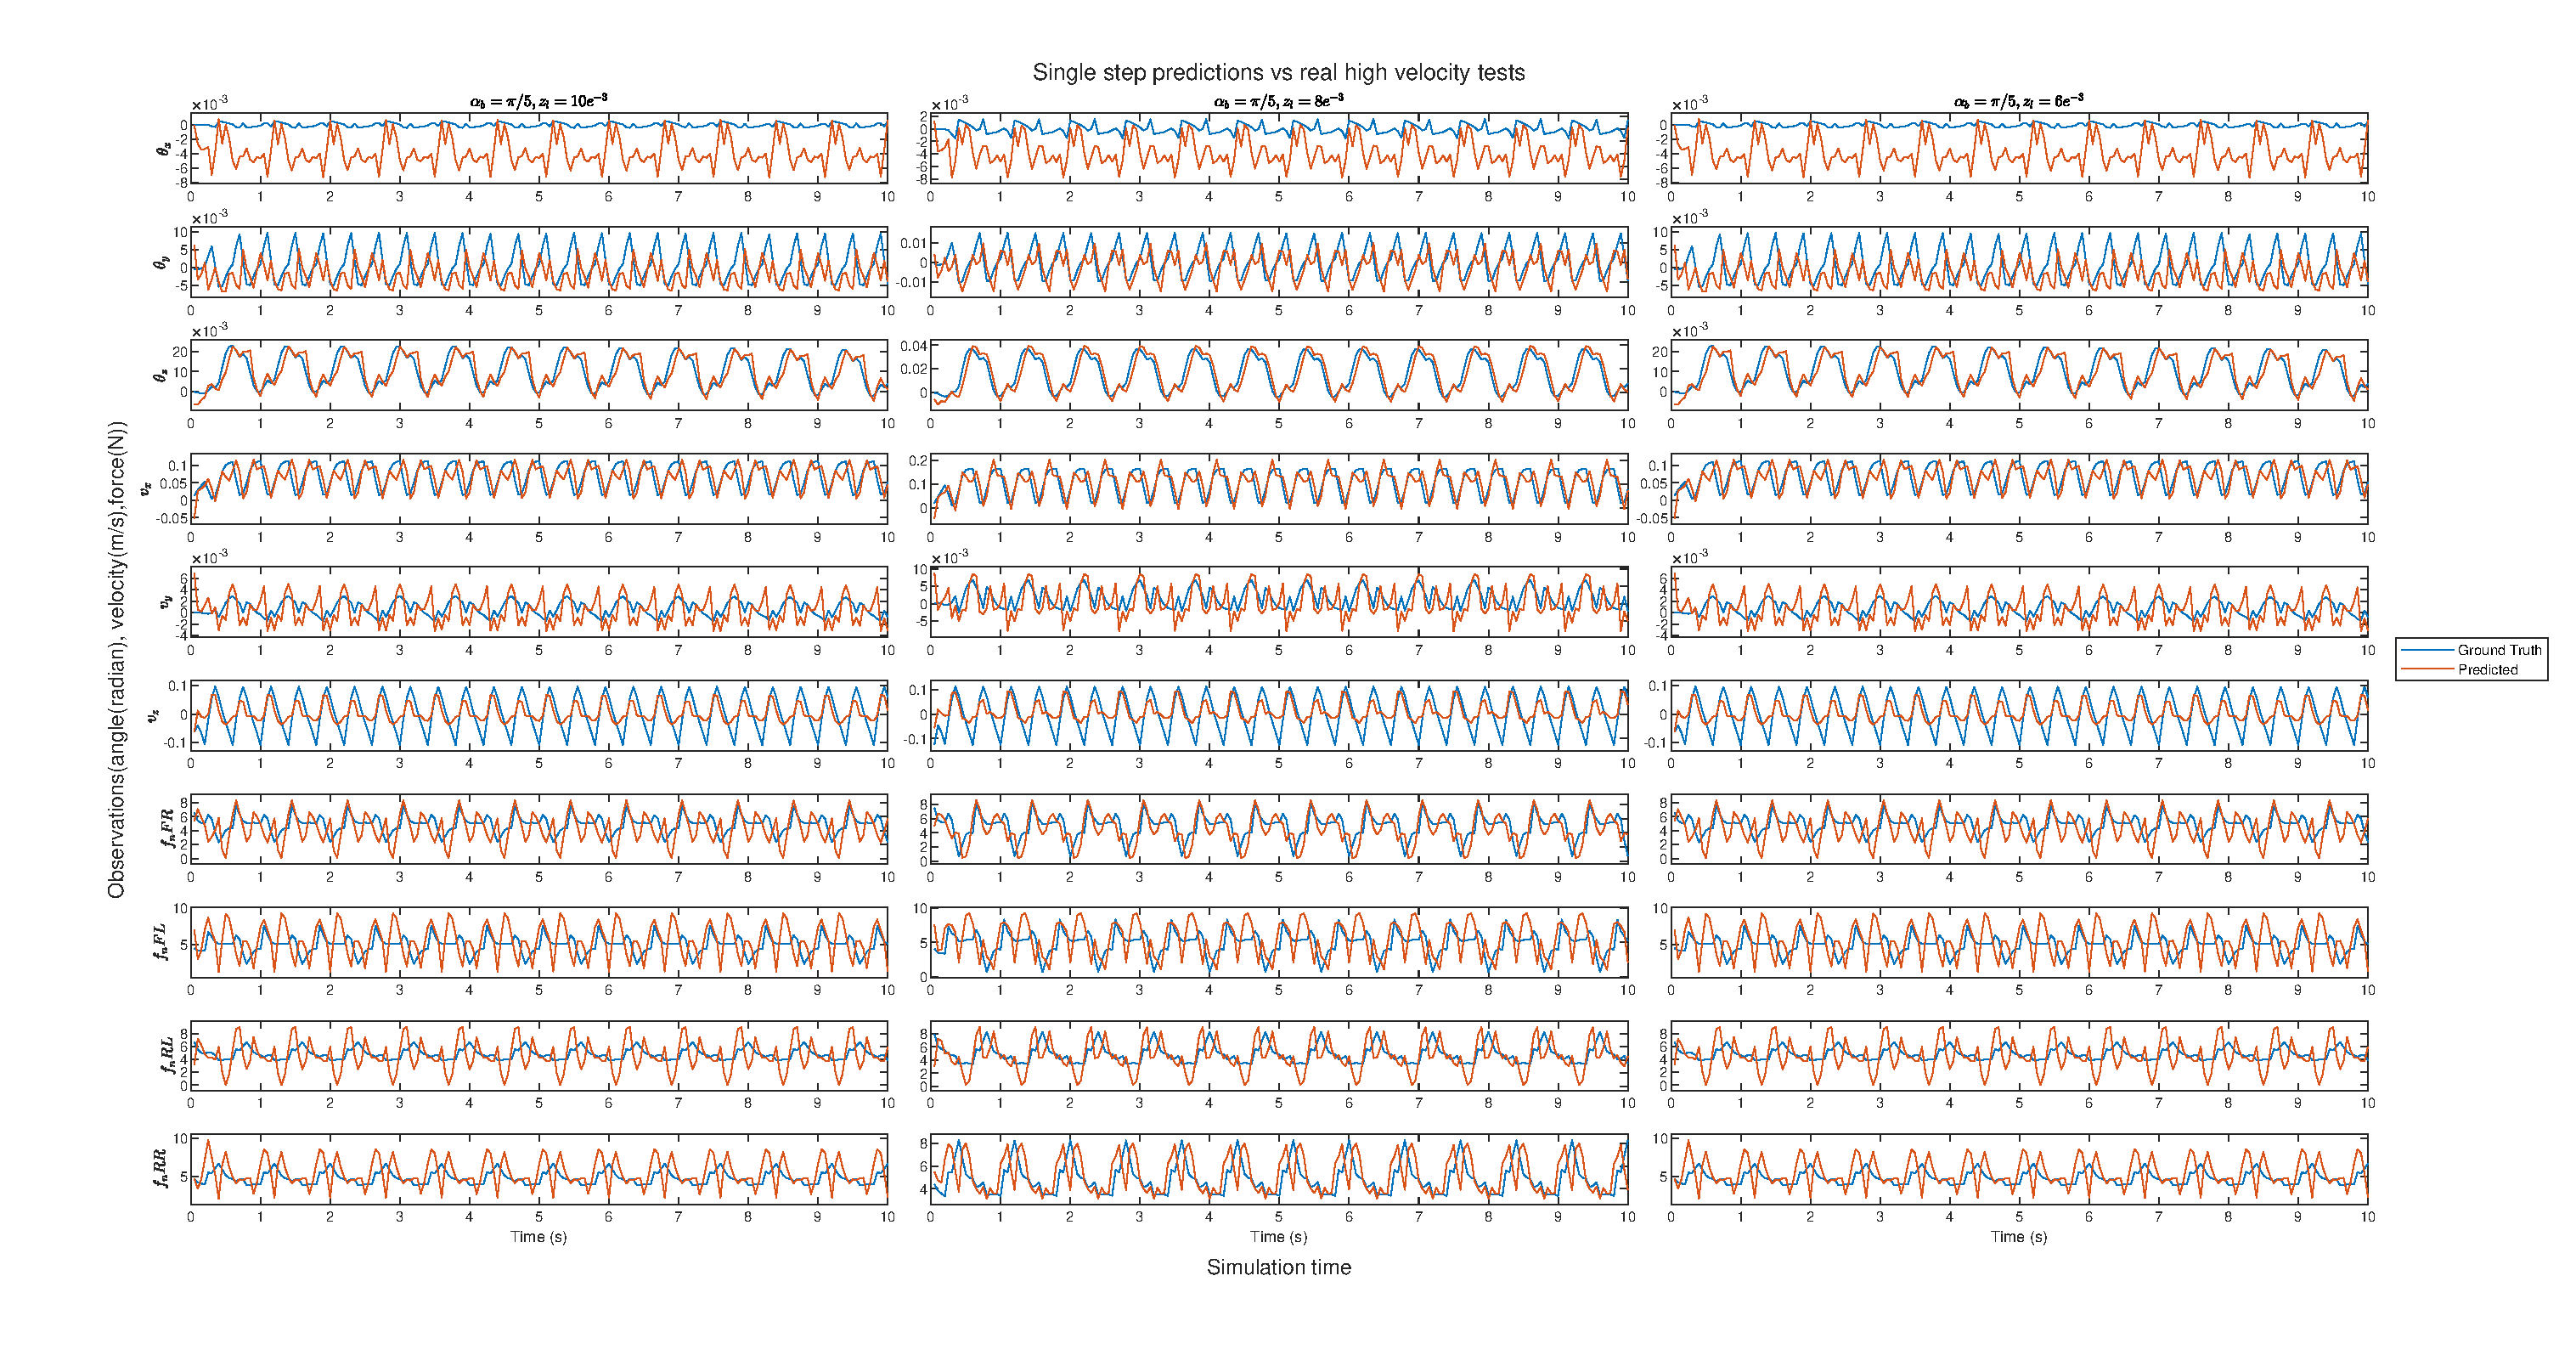
\includegraphics[width=\linewidth]{img/AppA/model_all.eps}
    \caption{Single step prediction test of DNN}
    \label{fig:DNN_test}
\end{figure}



\chapter{Source Code and Block Diagrams}
In this chapter, the main the source code and block diagrams implemented in Simulink is provided. These elements play a crucial role in this thesis, enabling the replication of experiments, validation of results, and the potential for further advancements in our work.


\section{Main Code of SoftQ}

\subsection*{Python Code for SoftQ}
The Python code for SoftQ can be found in here: \href{https://github.com/n7729697/KTH-MasterThesis/blob/main/code/SoftQ_optimized.py}{\faGithub\, \underline{Python Code}}

\subsection*{Matlab Code for MBRL}
\label{code:mbrl}
The Matlab code for MBRL training can be found in here: \href{https://github.com/n7729697/KTH-MasterThesis/blob/main/code/SoftQ_optimized.py}{\faGithub\,\underline{MATLAB Code}}

\section{Block Diagrams from Simulink}
\subsection*{Block Diagrams for MBRL}
The block diagrams for MBRL training and simulation in simulink could be found in here: \href{https://github.com/n7729697/KTH-MasterThesis/blob/main/img/AppB/it.pdf}{\faGithub\,\underline{ MBRL training block diagram}}
\subsection*{Block Diagrams for Continue Training and MFRL}

\subsection*{Block Diagrams for Simulink Controller}